\section{Introduction}
\seclabel{introduction}

Cloud-based Robotics and Automation systems exchange data and perform computation via networks instead of operating in isolation with limited computation and memory.
Potential advantages to using the Cloud include Big Data: access to updated libraries of images, maps, and object/product data; and Parallel Computation: access to parallel grid computing for statistical analysis, machine learning, and planning~\cite{kehoe2015survey}.
These benefits have recently been demonstrated in vision and speech, where datasets with millions of examples such as ImageNet have produced results~\cite{hannun2014deepspeech, krizhevsky2012imagenet} that surpass those obtained from decades of previous research.
This suggests that large-scale machine learning of grasps for vast numbers of possible object shapes, object poses, and environment configurations~\cite{goldfeder2011data, lenz2015deep, kappler2015leveraging}, could exhibit scaling effects similar to those observed in computer vision and speech recognition.

\begin{figure}[t!]
\centering
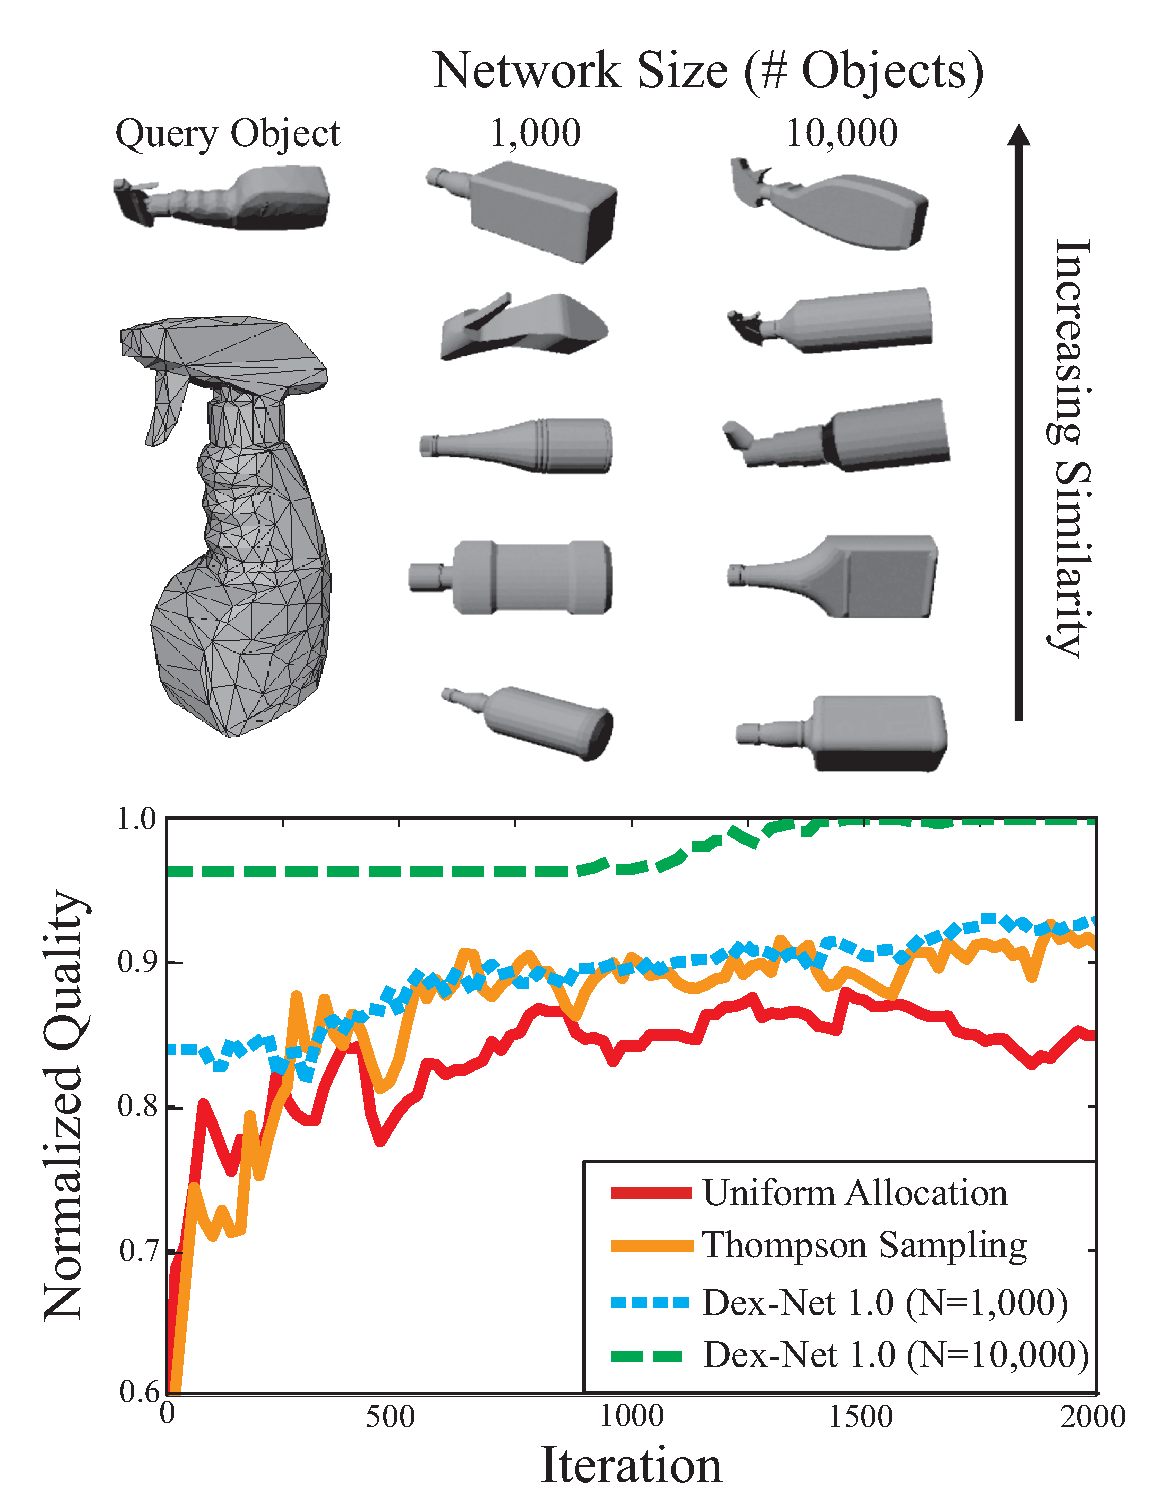
\includegraphics[scale=0.45]{figures/illustrations/spray_bottle_avg_reward_w_neighbors.eps}
\caption{Average normalized grasp quality versus iteration for 25 trials for the Dex-Net1.0 algorithm with 1,000 and 10,000 prior 3D objects from Dex-Net (bottom) and illustrations of five nearest neighbors in Dex-Net (top) for a spray bottle. We measure quality by the probability of force closure of the best grasp predicted by the algorithm on each iteration and compare with Thompson sampling without priors~\cite{laskey2015bandits} and uniform allocation~\cite{kehoe2012toward, weisz2012pose}. (Top) The spray bottle has no similar neighbors with 1,000 objects, but two other spray bottles are found by the MV-CNN in the 10,000 object set. (Bottom) As a result, the Dex-Net 1.0 algorithm quickly converges to the optimal grasp with 10,000 prior objects.}
\figlabel{avg-reward-spray}
\vspace*{-20pt}
\end{figure}

The primary contribution of this paper is the Dex-Net 1.0 algorithm for quickly finding a grasp with high probability of success for a binary grasp quality metric under uncertainty based on Multi-Armed Bandits (MABs).
The algorithm speeds up robust grasp planning by learning from a large dataset of prior grasps and 3D object models using Continuous Correlated Beta Processes (CCBPs)~\cite{goetschalckx2011continuous, montesano2012active}, an efficient model for predicting a distribution on the quality of each grasp from prior data.

To study scaling effects, we developed Dex-Net 1.0, a growing dataset that currently includes over 10,000 unique 3D object models selected to reflect objects that could be encountered in warehousing or the home such as containers, tools, tableware, and toys.
Dex-Net also contains approximately 2.5 million parallel-jaw grasps, as each object is labelled with up to 250 grasps and an estimate of the probability of force closure for each under uncertainty in object pose, gripper pose, and friction coefficient.
To the best of our knowledge, this is the largest object dataset used for grasping research to-date.
We incorporate Multi-View Convolutional Neural Networks (MV-CNNs)~\cite{su2015multi}, a state-of-the-art method for 3D shape classification, to efficiently retrieve similar 3D objects for predicting robust grasp quality with CCBPs.

We implement the Dex-Net 1.0 algorithm on Google Compute Engine and store Dex-Net 1.0 on Google Cloud Storage, with a system that can run up to 1,500 instances at once.
Experiments suggest that using 10,000 prior object models from Dex-Net reduces the number of samples needed to plan parallel-jaw grasps by up to 2$\times$ on average over 45 objects using the probability of force closure as a success metric.
%\TODO{Update with final results}

 





